\documentclass{article}

\usepackage[utf8]{inputenc}
\usepackage[french]{babel}
\usepackage[T1]{fontenc}
\usepackage{amsfonts}            %For \leadsto
\usepackage{amsmath}             %For \text
\usepackage{amssymb}              %For checkmark and x
\usepackage{fancybox}            %For \ovalbox
\usepackage{hyperref}
\usepackage{color}
\usepackage{enumitem}
\usepackage[margin=1in]{geometry}
\usepackage[parfill]{parskip}
\usepackage{graphicx}
\usepackage{float}
\usepackage{tikz}
\usepackage{listings}
\usepackage{xcolor}

\lstdefinelanguage{SQL}{
  keywords={SELECT, INSERT, UPDATE, DELETE, FROM, WHERE, AND, OR, NOT, NULL, LIKE, IN, CREATE, TABLE, PRIMARY, KEY, FOREIGN, REFERENCES, INT, VARCHAR, SERIAL, DATE, ON, DELETE},
  sensitive=false,
  morecomment=[l]{--},
  morestring=[b]',
}

\lstset{
  language=SQL,
  basicstyle=\ttfamily\footnotesize,
  keywordstyle=\color{blue}\bfseries,
  commentstyle=\color{gray}\itshape,
  stringstyle=\color{orange},
  numbers=left,
  numberstyle=\tiny\color{gray},
  stepnumber=1,
  numbersep=5pt,
  backgroundcolor=\color{white},
  showspaces=false,
  showstringspaces=false,
  frame=single,
  tabsize=2,
  captionpos=b,
  breaklines=true,
  breakatwhitespace=false
}
\usetikzlibrary{positioning, shapes.geometric, calc}

\newcommand \mML {\ensuremath\mu\textsl{ML}}
\newcommand \kw [1] {\textsf{#1}}
\newcommand \id [1] {\textsl{#1}}
\newcommand \punc [1] {\kw{`#1'}}
\newcommand \str [1] {\texttt{"#1"}}

\DeclareUnicodeCharacter{03BB}{\ensuremath{{\color{black}{\lambda}}}}

\graphicspath{ {./assets/images/} }

\title{Projet IFT2935}
\author{Olivier Larue (20269986) \\Claudéric DeRoy (20102789) \\Alexandre Toutant (20028191) \\Noah Tremblay Taillon (20190661)}

\begin{document}
\maketitle
\parskip = \baselineskip

\section{Modélisation en modèle E/A}

\begin{center}
  \begin{tikzpicture}[
    entity/.style={rectangle, draw=black, minimum width=2cm, minimum
      height=1cm},
    relation/.style={diamond, draw=black, aspect=2, inner sep=1pt},
    attr/.style={font=\small},
    key/.style={attr, font=\small\underline},
    line/.style={-}
    ]

    % Entités
    \node[entity] (Client) {Client};
    \node[entity, left=5cm of Client] (Livre) {Livre};
    

    % Calcul du milieu
    \path (Livre) -- (Client) coordinate[pos=0.5] (ClientLivreMid);
    
    % Relation
    \node[relation, above=2cm of ClientLivreMid] (Commande) {Commande};
    \node[relation, below=2cm of ClientLivreMid] (Emprunte) {Emprunte};
    \node[entity, right=3cm of Commande] (StatutCommande) {StatutCommande};
    \node[entity, left=3cm of Emprunte] (StatutEmprunt) {StatutEmprunt};
    
    % Attributs
    % Attr de Livre
    \node[attr, left=0.5cm of Livre] (isbn) {\underline{isbn}};
    \draw[line] (isbn) -- (Livre);

    \node[attr, above left=0.1cm of isbn] (titre) {titre};
    \draw[line] (titre) -- (Livre);

    \node[attr, above=0.1cm of titre] (genre) {genre};
    \draw[line] (genre) -- (Livre);

    \node[attr, right=0.1cm of genre] (auteur) {auteur};
    \draw[line] (auteur) -- (Livre);

    \node[attr, above=0.3cm of Livre] (nbExemplaire) {nbExemplaire};
    \draw[line] (nbExemplaire) -- (Livre);

    % Attr de Client
    \node[attr, right=0.5cm of Client] (idClient) {\underline{idClient}};
    \draw[line] (Client) -- (idClient);

    \node[attr, above=0.1cm of idClient] (permEmprunt) {permEmprunt};
    \draw[line] (Client) -- (permEmprunt);

    \node[attr, above left=0cm of permEmprunt] (nom) {nom};
    \draw[line] (Client) -- (nom);

    \node[attr, left=0cm of nom] (adresse) {adresse};
    \draw[line] (Client) -- (adresse);

    % Attr de Commande
    \node[attr, left=0.5cm of Commande] (idCommande)
    {\underline{idCommande}};
    \draw[line] (idCommande) -- (Commande);

    \node[attr, above=0.5cm of idCommande] (dateCommande) {dateCommande};
    \draw[line] (dateCommande) -- (Commande);

    \node[attr, right=0cm of dateCommande] (dateDispo) {dateDispo};
    \draw[line] (dateDispo) -- (Commande);

    \node[attr, right=0cm of dateDispo] (dateLimiteRetrait)
    {dateLimiteRetrait};
    \draw[line] (dateLimiteRetrait) -- (Commande);

    \node[attr, right=0cm of dateLimiteRetrait] (rang) {rang};
    \draw[line] (rang) -- (Commande);

    % Attr de StatutCommande
    \node[attr, above=0.5cm of StatutCommande] (statutCommande)
    {\underline{statutCommande}};
    \draw[line] (statutCommande) -- (StatutCommande);

    % Attr de Emprunte
    \node[attr, right=0.5cm of Emprunte] (idEmprunt) {\underline{idEmprunt}};
    \draw[line] (Emprunte) -- (idEmprunt);

    \node[attr, below=0.5cm of idEmprunt] (dateEmprunt) {dateEmprunt};
    \draw[line] (Emprunte) -- (dateEmprunt);

    \node[attr, left=0cm of dateEmprunt] (dateLimiteRetour) {dateLimiteRetour};
    \draw[line] (Emprunte) -- (dateLimiteRetour);
   
    % Attr de StatutEmprunt
    \node[attr, below=0.5cm of StatutEmprunt] (statutEmprunt)
    {\underline{statutEmprunt}};
    \draw[line] (StatutEmprunt) -- (statutEmprunt);

    % Liens entités-relations
    \draw[line] (Client) -- node[right] {0:3} (Commande);
    \draw[line] (Commande) -- node[above] {1:1} (StatutCommande);
    \draw[line] (Commande) -- node[left] {0:N} (Livre);
    \draw[line] (Livre) -- node[below] {0:N} (Emprunte);
    \draw[line] (Emprunte) -- node[right] {0:N} (Client);
    \draw[line] (StatutEmprunt) -- node[above] {1:1} (Emprunte);

  \end{tikzpicture}
\end{center}

Explications :
\begin{itemize}
\item \textbf{isbn et ids} : Ajoutés afin d'identifier facilement les
  différents éléments.
\item \textbf{Livre.nbExemplaire} : Représente le nombre d'exemplaires
  disponibles pour être emprunté. Par exemple, disons que la bibliothèque
  possède deux exemplaires du \textit{Multidictionnaire de la langue
    française}, et qu'un client à une commande ou emprunte directement ce
  livre, le nomnbre d'exemplaires disponibles sera diminué. Ceci explique aussi
  la cardinalité de la relation entre \textbf{Livre} et \textbf{Emprunte},
  puisqu'un livre avec plusieurs exemplaires peut donc être emprunté plusieurs
  fois en même temps.
\item \textbf{Commande.rang} : Représente le rang de cette commande parmi
  toutes les commandes sur le même livre. Disons que deux clients créent une
  commande pour le  \textit{Multidictionnaire de la langue française} alors
  qu'il n'y a qu'un seul exemplaire dans la bibliothèque, les commandes seront
  traitées selon la politique "première arrivée, première servie"
  (\textit{FIFO}). Le rang permet de savoir combien de commandes sont devant la
  notre.
\item \textbf{Commande.dateCommande} : Représente la date où la commande fut
  émise, dans le but d'ordonner la file d'attente.
\item \textbf{Commande.dateDispo et Commande.dateLimiteRetrait} : Utilent pour
  avoir un interval où le livre est réservé au client ayant fait cette
  commande. Ainsi, lorsque le livre commandé est disponible, ces deux attributs
  sont mis à jour. Si la date de limite de retrait est dépassée, alors la
  commande devient expirée et la priorité est donnée à la prochaine commande.
\item \textbf{StatutCommande.statutCommande} : Permet de faire l'énumération
  des statuts possibles pour une commande. Les statuts possibles pour une
  commande sont les suivants :
  \begin {itemize} [label=$\bullet$]
  \item En attente : La commande est passée, mais le client n'a pas encore la
    priorité sur ce document.
  \item Disponible pour le client : Le client à la priorité pour réserver ce
    document, pour une fenêtre de deux jours.
  \item Expirée : Le client avait la priorité pour réserver ce document, mais
    celui-ci a trop attendu. Il pert donc sa priorité et la commande n'est plus
    active.
  \item Annulée : Le client à décidé d'annuler la commander de son côté; la
    commande n'est plus active.
  \item Honorée : Le client à réservé ce document. La commande n'est plus
    active.
  \end{itemize}
  
\item \textbf{Client.permEmprunt} : Permet de vérifier si un client peut
  emprunter ou non. Par exemple, nous pourrions décider qu'un client ayant deux
  retards actifs serait interdit d'emprunter un troisième document jusqu'au
  règlement du retard.
\item \textbf{Client.adresse} : Afin de sauver de l'espace, nous n'avons pas
  représenté l'adresse comme étant un attribut complexe. Par contre, nous
  le décomposeront dans le modèle relationnel.
\item \textbf{StatutEmprunt.statutEmprunt} : Permet de faire l'énumération des
  statuts possibles pour un emprunt. Ceux-ci permettent de faire des
  statistiques sur les pratiques des clients. Les statuts possibles pour un
  emprunt sont les suivants :
  \begin{itemize}[label=$\bullet$]
  \item Retourné : Un emprunt est terminé, sans retard; celui-ci n'est
    plus actif et le livre redevient disponible.
  \item Réglé : Un emprunt était en retard, mais le client à réglé ce
    problème. L'emprunt n'est plus actif et le livre redevient disponible.
  \item En retard : Un emprunt est en retard; une action du client est
    nécessaire. Le livre est encore en possession du client.
  \item En cours : Un emprunt est en cours, sans retard. Le livre est encore en
    possession du client.
  \end{itemize}
  
\end{itemize}


\section{Transformation en modèle relationnel}
Explications :
\begin{itemize}
\item Pour commencer, toutes les entités faisant parties du modèle E/A seront
  conservées comme des tables différentes dans le modèle relationnel.
\item Puisque nous n'avons pas de relation 2D 1:1, les associations présentes
  dans le modèle E/A seront aussi présentes dans le modèle relationnel, tout en
  ayant des clés étrangères pour lier les entités concernées.
\item Afin de permettre d'avoir un client avec plusieurs adresses, et qu'une
  adresse puisse être partagée par plusieurs clients, nous avons créé les table
  \textbf{AdresseClient} et \textbf{Adresse}.
\item Afin de nous faciliter la vie plus tard avec la gestion des rangs des
  commandes, nous avons créé la table \textbf{RangCommande}.
\end{itemize}

Voici le modèle relationnel correspondant :
\begin{itemize}[label=$\bullet$]
\item Client(\underline{idClient}, permEmprunt, nom)
\item AdresseClient(\underline{\#idClient}, \underline{\#idAdresse})
\item Adresse(\underline{idAdresse}, rue, ville, code, pays)
\item Livre(\underline{isbn}, titre, genre, auteur, nbExemplaire)
\item StatutEmprunt(\underline{statutEmprunt})
\item StatutCommande(\underline{statutCommande})
\item Commande(\underline{idCommande}, \#isbn, \#idClient, \#statutCommande,
  dateCommande, dateDispo, \\
  dateLimiteRetrait)
\item RangCommande(\underline{\#idCommande}, \#isbn, rang)
\item Emprunte(\underline{idEmprunt}, \#isbn, \#idClient, \#statutEmprunt,
  dateEmprunt, dateLimiteRetour)
\end{itemize}

\section{Normalisation}
Pour la normalisation, nous normaliserons en 3NF. Pour les dépendances
fonctionnelles, nous laissons de côté les dépendances triviales.
\subsection{Client(\underline{idClient}, permEmprunt, nom)}
\subsubsection{Dépendances fonctionnelles}
Chaque client à un nom et potentiellement le droit d'emprunter des
livres. Donc, l'identifiant client permet de déterminer les deux autres.
$$idClient \rightarrow permEmprunt, \ nom$$

\subsubsection{3NF}
Comme nous avons déjà séparé \textbf{adresse} en d'autres relation, cette
relation est en 1NF; tous les attributs contiennent une valeur atomique (1NF).
Tout attribut non clé ne dépend pas d'une partie de la clé, donc cette relation
est 2NF. Tout attribut non clé dépend de la clé, donc cette relation est
3NF.


\subsection{AdresseClient(\underline{\#idClient}, \underline{\#idAdresse})}
\subsubsection{Dépendances fonctionnelles}
Aucune dépendance fonctionnelle non triviale ici, puisque qu'il n'y a pas d'attribut
non-clé.
\subsubsection{3NF}
Les attributs sont atomiques (1NF), ne dépendent pas d'une partie de la clé
(2NF), et dépendent directement de la clé (3NF).


\subsection{Adresse(\underline{idAdresse}, rue, ville, code, pays)}
\subsubsection{Dépendances fonctionnelles}
Chaque adresse à un identifiant unique permettant de retrouver ses
détails. Donc, cet identifiant permet de retrouver de manière unique les autres
attributs.
$$idAdresse \rightarrow rue, \ ville, \ code, \ pays$$

\subsubsection{3NF}
Les attributs sont atomiques (1NF), ne dépendent pas d'une partie de la clé
(2NF), et dépendent directement de la clé (3NF).


\subsection{Livre(\underline{isbn}, titre, genre, auteur, nbExemplaire)}
\subsubsection{Dépendances fonctionnelles}
Chaque livre a un identifiant unique. Plusieurs titres semblables peuvent
exister, et un auteur peut avoir écrit plusieurs livres. Donc, seul
l'identifiant unique d'un livre permet de déterminer les autres attributs.
$$isbn \rightarrow titre, \ genre, \ auteur, \ nbExemplaire$$

\subsubsection{3NF}
Les attributs sont atomiques (1NF), ne dépendent pas d'une partie de la clé
(2NF), et dépendent directement de la clé (3NF).


\subsection{StatutEmprunt(\underline{statutEmprunt}) et
  StatutCommande(\underline{statutCommande})}
\subsubsection{Dépendances fonctionnelles}
Ces deux relations n'ont qu'un seul attribut, donc aucune dépendance
fonctionnelle non triviale.

\subsubsection{3NF}
Les attributs sont atomiques (1NF), ne dépendent pas d'une partie de la clé
(2NF), et dépendent directement de la clé (3NF).


\subsection{Commande(\underline{idCommande}, \#isbn, \#idClient,
  \#statutCommande, dateCommande, dateDispo, dateLimiteRetrait)}
\subsubsection{Dépendances fonctionnelles}
L'identifiant unique permet de déterminer de manière unique les autres
attributs. Rien de dépend de l'isbn, car il peut y avoir plusieurs commandes
sur un même livre; un client peut faire jusqu'à trois commandes, donc il peut y
avoir plusieurs commandes pour un même client; il peut y avoir plusieurs
commandes pour une même date.
$$idCommande \rightarrow isbn, \ idClient, \ statutCommande, \ dateCommande, \
dateDispo, \ dateLimiteRetrait$$

\subsubsection{3NF}
Les attributs sont atomiques (1NF), ne dépendent pas d'une partie de la clé
(2NF), et dépendent directement de la clé (3NF).

\subsection{RangCommande(\underline{\#idCommande}, \#isbn, rang)}
\subsubsection{Dépendances fonctionnelles}
Puisqu'il peut y avoir plusieurs commandes avec un même rang (mais différents
livre), et qu'un livre peut avoir plusieurs commandes en attente, seul
l'identifiant de commande permet de trouver les deux autres attributs.
$$idCommande \rightarrow isbn, \ rang$$

\subsubsection{3NF}
Les attributs sont atomiques (1NF), ne dépendent pas d'une partie de la clé
(2NF), et dépendent directement de la clé (3NF).

\subsection{Emprunte(\underline{idEmprunt}, \#isbn, \#idClient,
  \#statutEmprunt, dateEmprunt, dateLimiteRetour)}
\subsubsection{Dépendances fonctionnelles}
Puisqu'il peut y avoir plusieurs exemplaires d'un même livre, l'isbn ne permet
par de déterminer un emprunt unique. Un client peut avoir plusieurs emprunts
(complétés ou actifs), et plusieurs emprunts peuvent afin le même statut; même
chose pour les dates. Donc, seul l'identifiant d'emprunt permet de déterminer
les autres attributs.
$$idEmprunt \rightarrow \ isbn, \ idClient,\ statutEmprunt, \ dateEmprunt, \
dateLimiteRetour$$

\subsubsection{3NF}
Les attributs sont atomiques (1NF), ne dépendent pas d'une partie de la clé
(2NF), et dépendent directement de la clé (3NF).

\subsection{Schéma final}
Le schéma n'a pas changé, puisque toutes les relations étaient déjà 3NF.
\begin{itemize}[label=$\bullet$]
\item Client(\underline{idClient}, permEmprunt, nom)
\item AdresseClient(\underline{\#idClient}, \underline{\#idAdresse})
\item Adresse(\underline{idAdresse}, rue, ville, code, pays)
\item Livre(\underline{isbn}, titre, genre, auteur, nbExemplaire)
\item StatutEmprunt(\underline{statutEmprunt})
\item StatutCommande(\underline{statutCommande})
\item Commande(\underline{idCommande}, \#isbn, \#idClient, \#statutCommande,
  dateCommande, dateDispo, \\
  dateLimiteRetrait)
\item RangCommande(\underline{\#idCommande}, \#isbn, rang)
\item Emprunte(\underline{idEmprunt}, \#isbn, \#idClient, \#statutEmprunt,
  dateEmprunt, dateLimiteRetour)
\end{itemize}

\section{Implémentation}
\subsection{Schéma des tables}
\begin{lstlisting}
-- Table Client
CREATE TABLE Client (
    idClient SERIAL PRIMARY KEY,
    permEmprunt VARCHAR(50),
    nom VARCHAR(100)
);

-- Table Adresse
CREATE TABLE Adresse (
    idAdresse SERIAL PRIMARY KEY,
    rue VARCHAR(255),
    ville VARCHAR(100),
    code VARCHAR(20),
    pays VARCHAR(100)
);

-- Table AdresseClient
CREATE TABLE AdresseClient (
    idClient INT,
    idAdresse INT,
    PRIMARY KEY (idClient, idAdresse),
    FOREIGN KEY (idClient) REFERENCES Client(idClient) ON DELETE CASCADE,
    FOREIGN KEY (idAdresse) REFERENCES Adresse(idAdresse) ON DELETE CASCADE
);

-- Table Livre
CREATE TABLE Livre (
    isbn VARCHAR(20) PRIMARY KEY,
    titre VARCHAR(255),
    genre VARCHAR(50),
    auteur VARCHAR(100),
    nbExemplaire INT
);

-- Table StatutEmprunt
CREATE TABLE StatutEmprunt (
    statutEmprunt VARCHAR(50) PRIMARY KEY
);

-- Table StatutCommande
CREATE TABLE StatutCommande (
    statutCommande VARCHAR(50) PRIMARY KEY
);

-- Table Commande
CREATE TABLE Commande (
    idCommande SERIAL PRIMARY KEY,
    isbn VARCHAR(20),
    idClient INT,
    statutCommande VARCHAR(50),
    dateCommande DATE,
    dateDispo DATE,
    dateLimiteRetrait DATE,
    FOREIGN KEY (isbn) REFERENCES Livre(isbn),
    FOREIGN KEY (idClient) REFERENCES Client(idClient),
    FOREIGN KEY (statutCommande) REFERENCES StatutCommande(statutCommande)
);

-- Table RangCommande
CREATE TABLE RangCommande (
    idCommande INT,
    isbn VARCHAR(20),
    rang INT,
    PRIMARY KEY (idCommande, isbn),
    FOREIGN KEY (idCommande) REFERENCES Commande(idCommande) ON DELETE CASCADE,
    FOREIGN KEY (isbn) REFERENCES Livre(isbn)
);

-- Table Emprunte
CREATE TABLE Emprunte (
    idEmprunt SERIAL PRIMARY KEY,
    isbn VARCHAR(20),
    idClient INT,
    statutEmprunt VARCHAR(50),
    dateEmprunt DATE,
    dateLimiteRetour DATE,
    FOREIGN KEY (isbn) REFERENCES Livre(isbn),
    FOREIGN KEY (idClient) REFERENCES Client(idClient),
    FOREIGN KEY (statutEmprunt) REFERENCES StatutEmprunt(statutEmprunt)
);

\end{lstlisting}

\subsection{Population des tables}
\begin{lstlisting}
  -- Insertion dans Client
INSERT INTO Client (idClient, permEmprunt, nom) VALUES
(1, 'PERM0001', 'Client_1'),
(2, 'PERM0002', 'Client_2'),
(3, 'PERM0003', 'Client_3'),
(4, 'PERM0004', 'Client_4'),
(5, 'PERM0005', 'Client_5'),
(6, 'PERM0006', 'Client_6'),
(7, 'PERM0007', 'Client_7'),
(8, 'PERM0008', 'Client_8'),
(9, 'PERM0009', 'Client_9'),
(10, 'PERM0010', 'Client_10');

-- Insertion dans Adresse
INSERT INTO Adresse (idAdresse, rue, ville, code, pays) VALUES
(1, '1 rue Exemple', 'Ville_1', 'H0001', 'Canada'),
(2, '2 rue Exemple', 'Ville_2', 'H0002', 'Canada'),
(3, '3 rue Exemple', 'Ville_3', 'H0003', 'Canada'),
(4, '4 rue Exemple', 'Ville_4', 'H0004', 'Canada'),
(5, '5 rue Exemple', 'Ville_0', 'H0005', 'Canada'),
(6, '6 rue Exemple', 'Ville_1', 'H0006', 'Canada'),
(7, '7 rue Exemple', 'Ville_2', 'H0007', 'Canada'),
(8, '8 rue Exemple', 'Ville_3', 'H0008', 'Canada'),
(9, '9 rue Exemple', 'Ville_4', 'H0009', 'Canada'),
(10, '10 rue Exemple', 'Ville_0', 'H0010', 'Canada');

-- Insertion dans AdresseClient
INSERT INTO AdresseClient (idClient, idAdresse) VALUES
(1, 1),
(2, 2),
(3, 3),
(4, 4),
(5, 5),
(6, 6),
(7, 7),
(8, 8),
(9, 9),
(10, 10);

-- Insertion dans Livre
INSERT INTO Livre (isbn, titre, genre, auteur, nbExemplaire) VALUES
('ISBN0001', 'Titre_1', 'Roman', 'Auteur_1', 6),
('ISBN0002', 'Titre_2', 'Science', 'Auteur_2', 9),
('ISBN0003', 'Titre_3', 'Roman', 'Auteur_3', 2),
('ISBN0004', 'Titre_4', 'Histoire', 'Auteur_4', 7),
('ISBN0005', 'Titre_5', 'Roman', 'Auteur_5', 8),
('ISBN0006', 'Titre_6', 'Histoire', 'Auteur_6', 3),
('ISBN0007', 'Titre_7', 'Science', 'Auteur_7', 6),
('ISBN0008', 'Titre_8', 'Roman', 'Auteur_8', 1),
('ISBN0009', 'Titre_9', 'Science', 'Auteur_9', 4),
('ISBN0010', 'Titre_10', 'Roman', 'Auteur_10', 7);

-- Insertion dans StatutEmprunt
INSERT INTO StatutEmprunt (statutEmprunt) VALUES
('en_cours'),
('retourne'),
('retard');

-- Insertion dans StatutCommande
INSERT INTO StatutCommande (statutCommande) VALUES
('en_attente'),
('disponible'),
('recuperee');

-- Insertion dans Commande
INSERT INTO Commande (idCommande, isbn, idClient, statutCommande, dateCommande, dateDispo, dateLimiteRetrait) VALUES
(1, 'ISBN0002', 1, 'recuperee', '2025-04-15', '2025-04-16', '2025-04-22'),
(2, 'ISBN0003', 2, 'en_attente', '2025-04-13', '2025-04-15', '2025-04-22'),
(3, 'ISBN0004', 3, 'disponible', '2025-04-11', '2025-04-14', '2025-04-22'),
(4, 'ISBN0005', 4, 'en_attente', '2025-04-09', '2025-04-13', '2025-04-22'),
(5, 'ISBN0006', 5, 'recuperee', '2025-04-07', '2025-04-12', '2025-04-22'),
(6, 'ISBN0007', 6, 'disponible', '2025-04-05', '2025-04-11', '2025-04-22'),
(7, 'ISBN0008', 7, 'en_attente', '2025-04-03', '2025-04-10', '2025-04-22'),
(8, 'ISBN0009', 8, 'recuperee', '2025-04-01', '2025-04-09', '2025-04-22'),
(9, 'ISBN0010', 9, 'disponible', '2025-03-30', '2025-04-08', '2025-04-22'),
(10, 'ISBN0001', 10, 'en_attente', '2025-03-28', '2025-04-07', '2025-04-22');

-- Insertion dans RangCommande
INSERT INTO RangCommande (idCommande, isbn, rang) VALUES
(1, 'ISBN0002', 3),
(2, 'ISBN0003', 1),
(3, 'ISBN0004', 2),
(4, 'ISBN0005', 5),
(5, 'ISBN0006', 1),
(6, 'ISBN0007', 2),
(7, 'ISBN0008', 4),
(8, 'ISBN0009', 1),
(9, 'ISBN0010', 2),
(10, 'ISBN0001', 3);

-- Insertion dans Emprunte
INSERT INTO Emprunte (idEmprunt, isbn, idClient, statutEmprunt, dateEmprunt, dateLimiteRetour) VALUES
(1, 'ISBN0002', 1, 'retourne', '2025-03-27', '2025-04-29'),
(2, 'ISBN0003', 2, 'en_cours', '2025-03-18', '2025-04-22'),
(3, 'ISBN0004', 3, 'retard', '2025-04-12', '2025-05-06'),
(4, 'ISBN0005', 4, 'en_cours', '2025-03-08', '2025-04-22'),
(5, 'ISBN0006', 5, 'retourne', '2025-04-07', '2025-05-07'),
(6, 'ISBN0007', 6, 'retard', '2025-04-09', '2025-05-01'),
(7, 'ISBN0008', 7, 'retourne', '2025-03-18', '2025-05-01'),
(8, 'ISBN0009', 8, 'en_cours', '2025-04-05', '2025-05-05'),
(9, 'ISBN0010', 9, 'retard', '2025-04-11', '2025-05-01'),
(10, 'ISBN0001', 10, 'en_cours', '2025-03-30', '2025-05-03');
\end{lstlisting}

\section{Question/reponse}
\subsection*{1. Lister les clients qui ont au moins un emprunt en retard}

\textbf{SQL :}
\begin{lstlisting}
SELECT e.idClient, c.nom, COUNT(*) AS nbRetards
FROM Emprunte e
JOIN Client c USING (idClient)
WHERE e.statutEmprunt = 'retard'
GROUP BY e.idClient, c.nom;
\end{lstlisting}

\textbf{Algèbre relationnelle :}
\[
\pi_{idClient, nom, \text{count}(*)} \left(
  \sigma_{statutEmprunt = 'retard'}(Emprunte) \bowtie Client
\right)
\]

\textbf{Optimisation :}
\begin{itemize}
  \item La condition \texttt{statutEmprunt = 'retard'} est appliquée avant la jointure, ce qui réduit les lignes traitées.
  \item L’opérateur \texttt{JOIN USING} est plus concis lorsque les noms de colonnes sont identiques (\texttt{idClient}).
  \item L’utilisation de \texttt{COUNT(*)} évite de devoir vérifier la nullité d’un champ et est plus efficace.
  \item Aucune clause \texttt{HAVING} n’est nécessaire, car la condition est déjà garantie par le \texttt{WHERE}.
\end{itemize}

\bigskip

\subsection*{2. Lister les emprunts actifs par client avec la date limite de retour}

\textbf{SQL :}
\begin{lstlisting}
SELECT e.idEmprunt, c.nom, l.titre, e.dateEmprunt, e.dateLimiteRetour
FROM Emprunte e
JOIN Client c USING (idClient)
JOIN Livre l USING (isbn)
WHERE e.statutEmprunt = 'en_cours'
ORDER BY e.dateLimiteRetour;
\end{lstlisting}

\textbf{Algèbre relationnelle :}
\[
\pi_{idEmprunt, nom, titre, dateEmprunt, dateLimiteRetour} \left(
  \sigma_{statutEmprunt = 'en\_cours'}(Emprunte \bowtie Client \bowtie Livre)
\right)
\]

\textbf{Optimisation :}
\begin{itemize}
  \item Le filtrage des emprunts en cours est appliqué dès le départ.
  \item Les jointures utilisent l’opérateur \texttt{USING} pour plus de clarté et d’efficacité.
  \item Le tri est effectué uniquement sur une colonne déjà présente, sans transformation ou calcul.
\end{itemize}

\bigskip

\subsection*{3. Lister les commandes non récupérées à une date donnée}

\textbf{SQL :}
\begin{lstlisting}
SELECT c.idCommande, cl.nom, l.titre, c.dateCommande, c.dateLimiteRetrait, c.statutCommande
FROM Commande c
JOIN Client cl USING (idClient)
JOIN Livre l USING (isbn)
WHERE c.statutCommande IN ('en_attente', 'disponible')
AND c.dateLimiteRetrait >= DATE '2025-04-17'
ORDER BY c.dateLimiteRetrait;
\end{lstlisting}

\textbf{Algèbre relationnelle :}
\begin{align*}
  \pi_{idCommande, nom, titre, dateCommande, dateLimiteRetrait, statutCommande} \Big( \ 
    &\sigma_{\substack{
      statutCommande \in \{en\_attente,\ disponible\} \\
      \land\ dateLimiteRetrait \geq 2025\text{-}04\text{-}17
    }} \Big( \\
    &\hspace{1em} Commande \ \bowtie\ Client \ \bowtie\ Livre \Big) \Big)
\end{align*}

\textbf{Optimisation :}
\begin{itemize}
  \item Les lignes sont filtrées en amont selon deux conditions restrictives : le statut et la date limite.
  \item L’usage explicite du type \texttt{DATE} assure une comparaison efficace et sans conversion implicite.
  \item La requête ne sélectionne que les colonnes nécessaires à l’affichage.
\end{itemize}

\bigskip

\subsection*{4. Compter le nombre total de commandes par genre de livre}

\textbf{SQL :}
\begin{lstlisting}
SELECT l.genre, COUNT(*) AS nbCommandes
FROM Commande c
JOIN Livre l USING (isbn)
GROUP BY l.genre
ORDER BY nbCommandes DESC;
\end{lstlisting}

\textbf{Algèbre relationnelle :}
\[
\gamma_{genre, \text{count}(*)}(Commande \bowtie Livre)
\]

\textbf{Optimisation :}
\begin{itemize}
  \item Le regroupement est fait uniquement sur le champ \texttt{genre}, ce qui simplifie le plan d’exécution.
  \item L’utilisation de \texttt{COUNT(*)} est plus performante pour le comptage global.
  \item L’ordre décroissant est appliqué sur une agrégation déjà calculée, sans besoin de calcul supplémentaire.
\end{itemize}

\section{Développement}
Le projet a été conçu comme une application full stack. Le front-end a été développé avec React, un framework JavaScript qui facilite le développement d'interfaces. Pour le back-end, nous avons utilisé Express.js, un framework léger et rapide à prendre en main.

Le tout est hébergé dans un répertoire GitHub, incluant le front-end, le back-end, ainsi que les scripts nécessaires à la base de données. Nous avons choisi de tout centraliser dans un seul dépôt étant donné la petite taille du projet, ce qui simplifie la gestion et la collaboration.

Nous avons utilisé Sequelize comme ORM pour faciliter les requêtes entre Express.js et la base de données PostgreSQL. Sequelize s’intègre bien à l’environnement JavaScript, ce qui a renforcé notre choix.

La base de données est gérée dans un conteneur Docker, via un script Docker Compose. Ce dernier configure automatiquement un serveur PostgreSQL local, dont les données sont initialement populées à l’aide d’un fichier seed.sql, permettant à chaque utilisateur d’avoir les mêmes données initiales.

Pour faciliter l’installation et l'exécution du projet, un fichier README.md détaille les étapes nécessaires. Le développement a été effectué avec Visual Studio Code, en s’appuyant sur la documentation officielle de chaque technologie.

\textbf{Par exemple :}
\begin{itemize}
    \item Pour Express.js : expressjs.com/en/starter/installing.html
    \item Pour React : react.dev/learn/installation et react.dev/learn
    \item Pour Sequelize : https://sequelize.org/docs/v6/getting-started/
\end{itemize}


\textbf{Le projet comporte 5 pages:}
\begin{itemize}
    \item La page d'acceuil (HomePage)
    \item Pages 1-4. Une page pour chaque questions
\end{itemize}

\textbf{L'api du backend comporte sur 5 routes: }
\begin{itemize}
    \item http://localhost:5000/api  (pour verifier si l'api fonctionne. Route de base de l'api.)
    \item http://localhost:5000/api/question1 (pour obtenir le contenu en format JSON de la requête pour la question 1)
    \item http://localhost:5000/api/question2 (pour obtenir le contenu en format JSON de la requête pour la question 2)
    \item http://localhost:5000/api/question3 (pour obtenir le contenu en format JSON de la requête pour la question 3)
    \item http://localhost:5000/api/question4 (pour obtenir le contenu en format JSON de la requête pour la question 4)
\end{itemize}

Une fois le projet lancé et que vous accédez à \texttt{localhost:5173}, vous arrivez sur la page d’accueil de l'application :
\begin{figure}[H]
    \centering
    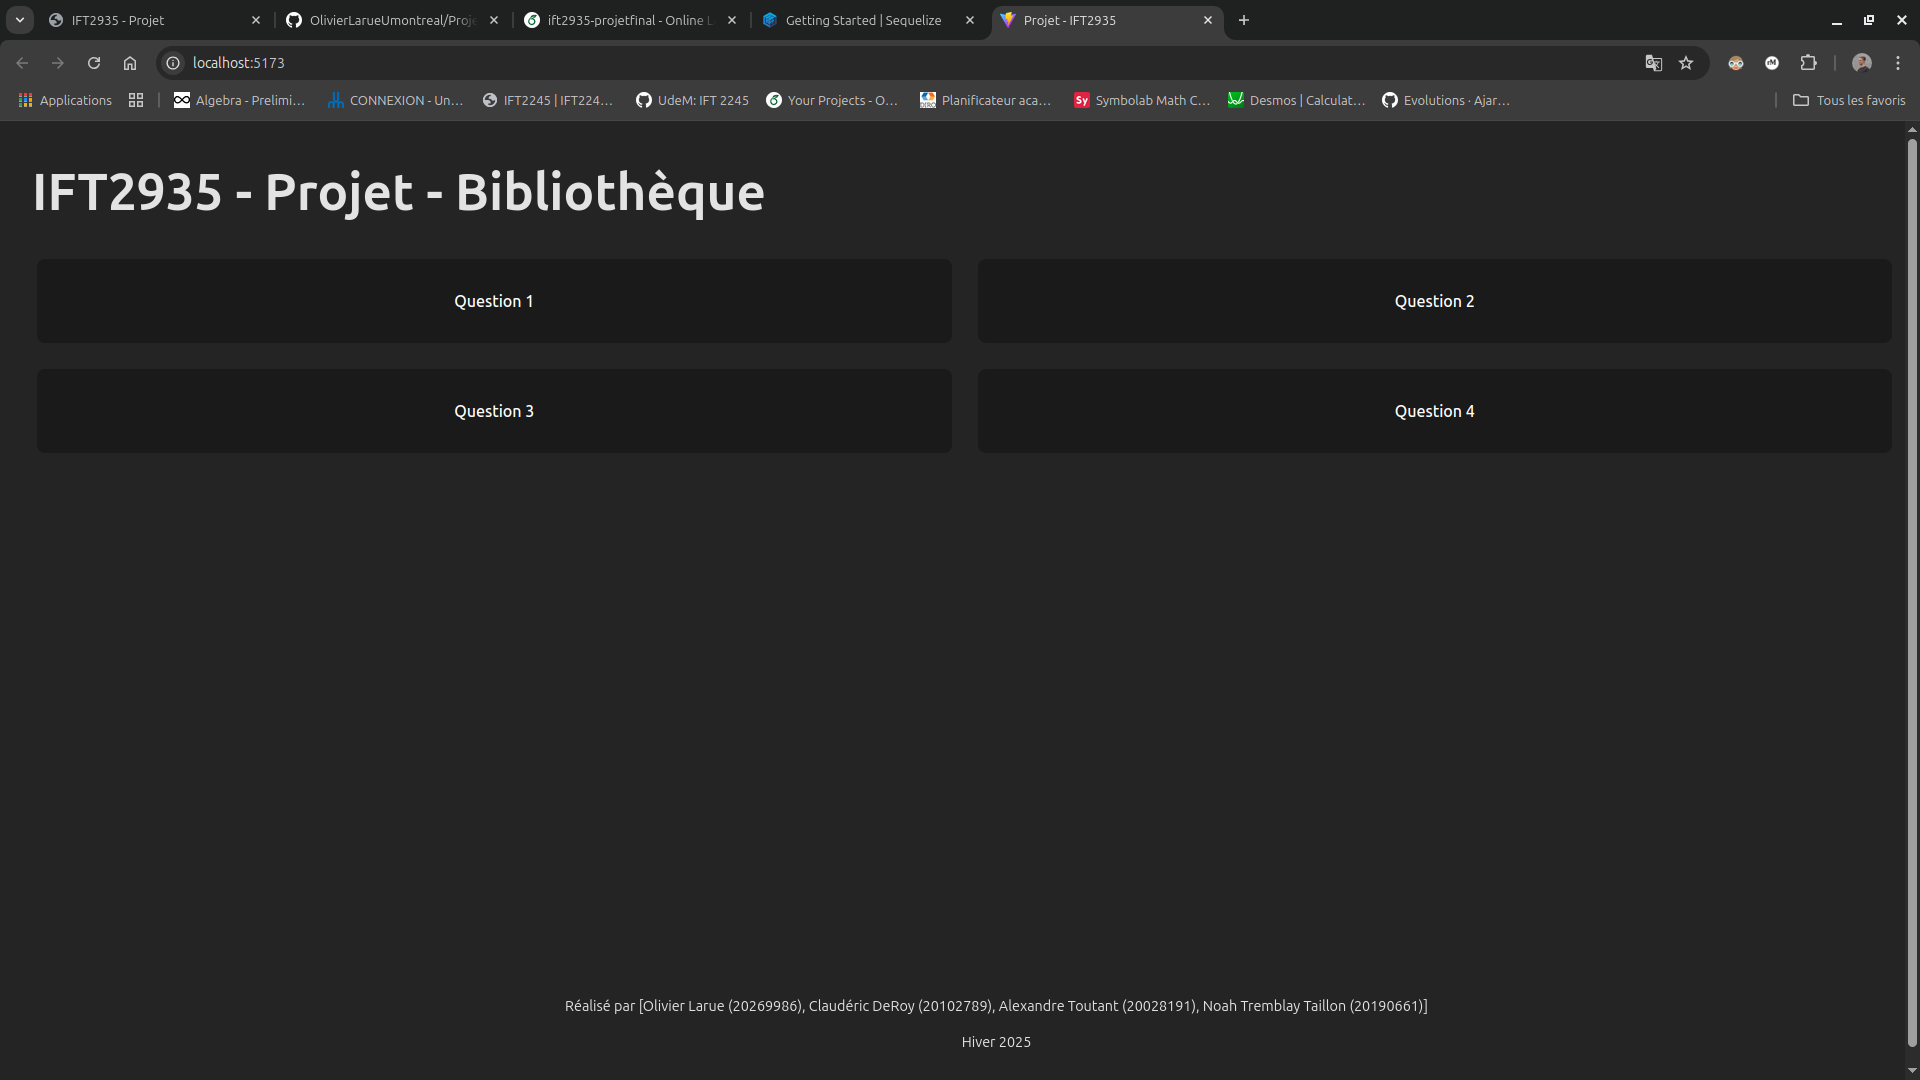
\includegraphics[width=1\textwidth]{projetHomePage.png}
    \label{fig:}
\end{figure}

La page d’accueil contient quatre boutons, chacun représentant une question que nous avons formulée précédemment. Lorsqu’on clique sur l’un de ces boutons, la page affiche :
\begin{itemize}
    \item la question sélectionnée,
    \item la requête SQL correspondante,
    \item le résultat de cette requête.
\end{itemize}

Par exemple, pour la question 1, voici ce que l’on obtient : 
\begin{figure}[H]
    \centering
    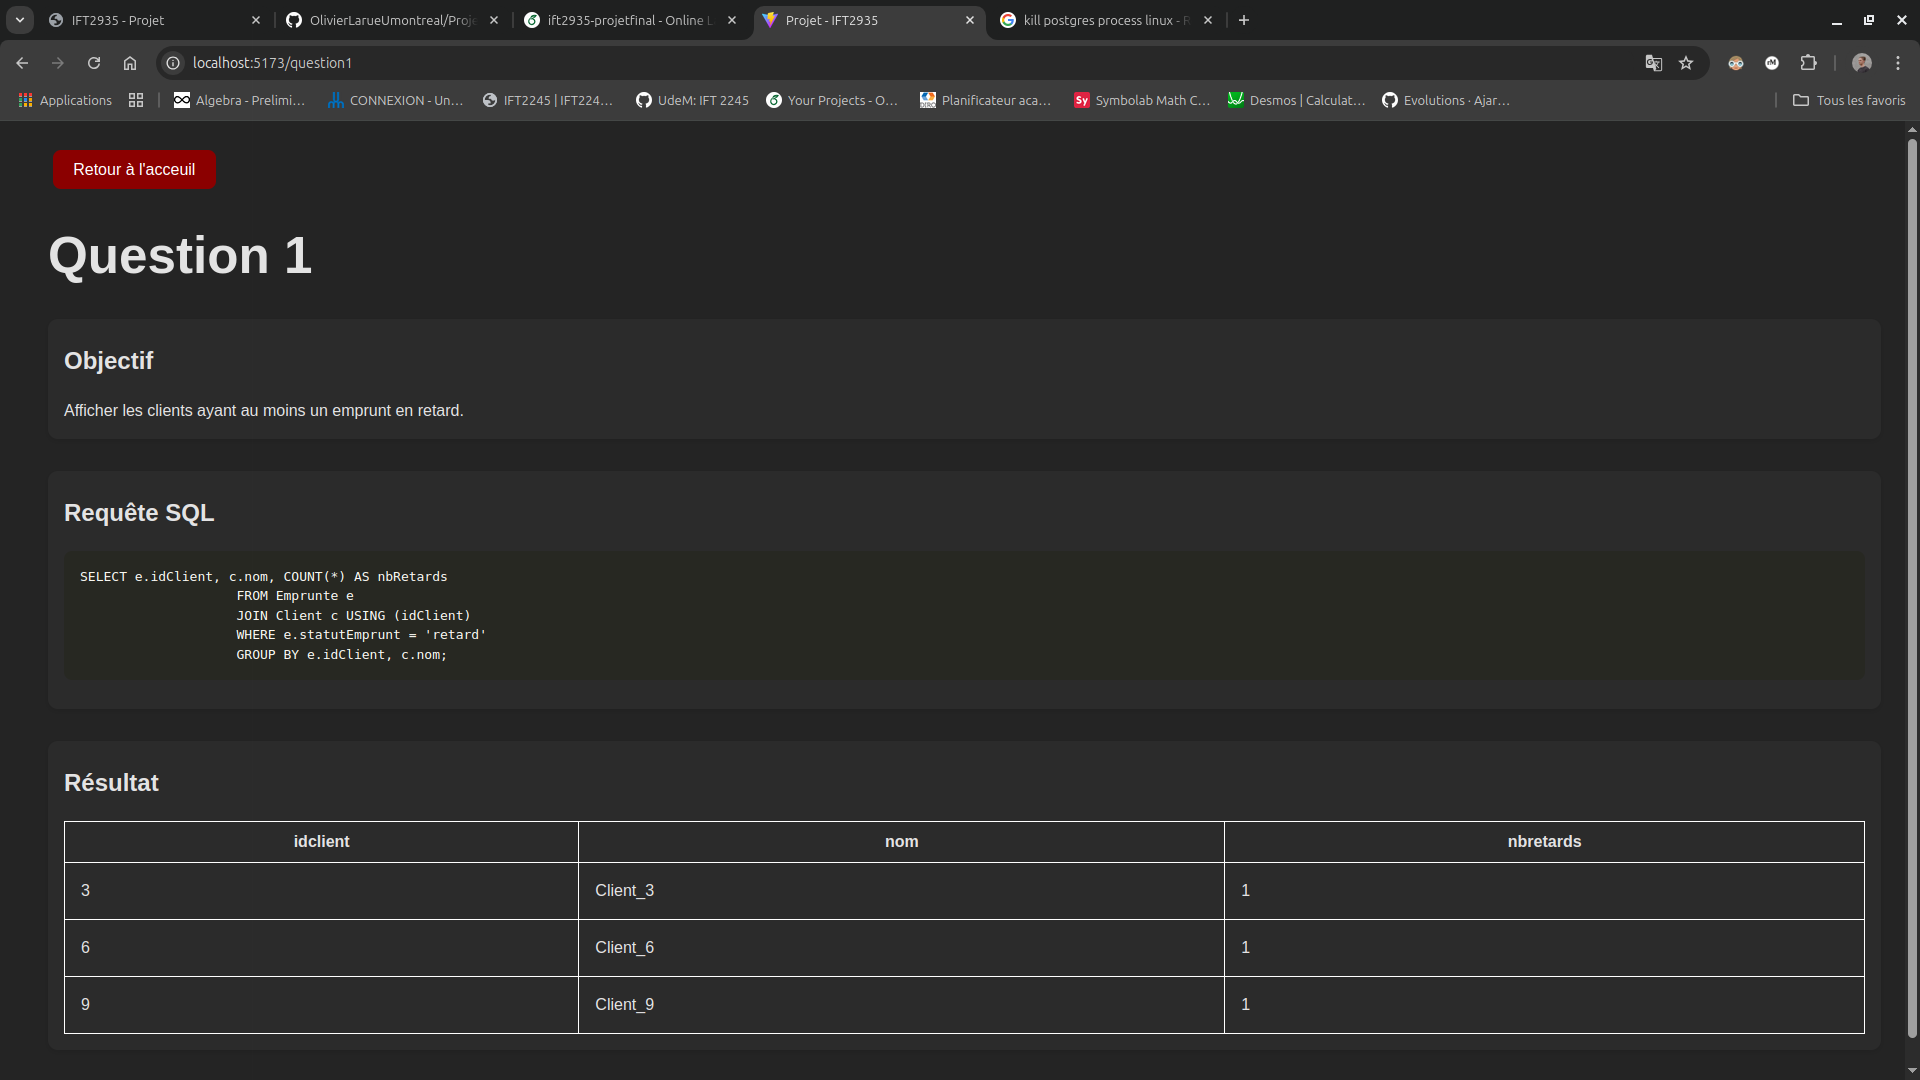
\includegraphics[width=1\textwidth]{projetQuestion1.png}
    \label{fig:}
\end{figure}

La même logique s’applique pour les quatre questions : chaque page est dédiée à une question spécifique et affiche la question, la requête SQL utilisée, ainsi que le résultat obtenu.

\section{Installation}
Une \href{file:./promenade_projet_ift_2935_groupe_20.mp4}{vidéo} ainsi que des instructions dans un \href{https://github.com/OlivierLarueUmontreal/ProjetIFT2935}{dépôt} GitHub expliquent comment procéder pour l'installation et l'exécution du projet.

\end{document}
